% LaTeX Präsentationsvorlage (2013) der TU Graz, rev12, 2013/01/31
% !TeX encoding = UTF-8
\documentclass{beamer}
% \documentclass[aspectratio=169]{beamer}
% \usetheme{tugraz2013}
% \usetheme[notes]{tugraz2013}
\usepackage{../common/beamerthemetugraz2013}
\usepackage{color}
\usepackage{multicol}
\usepackage{bbding}
\usepackage{wasysym}
\usepackage{caption}
\usepackage{tikz}
\usetikzlibrary{shapes.multipart, positioning}
% \usepackage{minted}

\usepackage{listings}
\usepackage{xcolor}

\definecolor{codegreen}{rgb}{0,0.6,0}
\definecolor{codegray}{rgb}{0.5,0.5,0.5}
\definecolor{codepurple}{rgb}{0.58,0,0.82}
\definecolor{backcolour}{rgb}{0.95,0.95,0.92}
\lstdefinestyle{mystyle}{
    backgroundcolor=\color{backcolour},   
    commentstyle=\color{codegreen},
    keywordstyle=\color{magenta},
    numberstyle=\tiny\color{codegray},
    stringstyle=\color{codepurple},
    basicstyle=\ttfamily\footnotesize,
    breakatwhitespace=false,         
    breaklines=true,                 
    captionpos=b,                    
    keepspaces=true,                 
    numbers=left,                    
    numbersep=5pt,                  
    showspaces=false,                
    showstringspaces=false,
    showtabs=false,                  
    tabsize=2
}

\lstset{style=mystyle}

\usepackage{picture}
\usepackage{rotating}

\definecolor{darkred}{rgb}{0.85,0.16,0.0}
\definecolor{darkgreen}{rgb}{0.16,0.70,0.27}

\newcommand{\hrefu}[2]{\underline{\href{#1}{#2}}}

\newcommand{\red}[1]{{\color{red} #1}}
\newcommand{\blue}[1]{{\color{blue} #1}}
\newcommand{\darkgreen}[1]{\textcolor{darkgreen}{#1}}
\newcommand{\darkred}[1]{\textcolor{darkred}{#1}}

\newcommand*{\vpointer}{\vcenter{\hbox{\scalebox{1.5}{\large\pointer}}}}

\newcommand{\be}[1]{\begin{equation} \label{#1}}
\newcommand{\ee}{\end{equation}}
\newcommand{\bea}[1]{\begin{eqnarray} \label{#1}}
\newcommand{\eea}{\end{eqnarray}}
\newcommand{\bean}{\begin{eqnarray*}}
\newcommand{\eean}{\end{eqnarray*}}

\newcommand{\non}{\nonumber\\}
\newcommand{\eq}[1]{(\ref{#1})}
\newcommand{\difp}[2]{\frac{\partial #1}{\partial #2}}
\newcommand{\br}{{\bf r}}
\newcommand{\bR}{{\bf R}}
\newcommand{\bA}{{\bf A}}
\newcommand{\bB}{{\bf B}}
\newcommand{\bE}{{\bf E}}
\newcommand{\bm}{{\bf m}}
%\renewcommand{\bm}{{\bf m}}
\newcommand{\bn}{{\bf n}}
\newcommand{\bN}{{\bf N}}
\newcommand{\bp}{{\bf p}}
\newcommand{\bP}{{\bf P}}
\newcommand{\bF}{{\bf F}}
\newcommand{\by}{{\bf y}}
\newcommand{\bz}{{\bf z}}
\newcommand{\bZ}{{\bf Z}}
\newcommand{\bV}{{\bf V}}
\newcommand{\bv}{{\bf v}}
\newcommand{\bu}{{\bf u}}
\newcommand{\bx}{{\bf x}}
\newcommand{\bX}{{\bf X}}
\newcommand{\bW}{{\bf W}}
\newcommand{\bJ}{{\bf J}}
\newcommand{\bj}{{\bf j}}
\newcommand{\bk}{{\bf k}}
\newcommand{\bTheta}{{\bf \Theta}}
\newcommand{\btheta}{{\boldsymbol\theta}}
\newcommand{\bOmega}{{\bf \Omega}}
\newcommand{\bomega}{{\boldsymbol\omega}}
\newcommand{\brho}{{\boldsymbol\rho}}
\newcommand{\rd}{{\rm d}}
\newcommand{\rJ}{{\rm J}}
\newcommand{\ph}{{\varphi}}
\newcommand{\te}{\theta}
\newcommand{\tht}{\vartheta}
\newcommand{\vpar}{v_\parallel}
\newcommand{\vparkb}{v_{\parallel k b}}
\newcommand{\vparkm}{v_{\parallel k m}}
\newcommand{\Jpar}{J_\parallel}
\newcommand{\ppar}{p_\parallel}
\newcommand{\Bpstar}{B_\parallel^*}
\newcommand{\intpi}{\int\limits_{0}^{2\pi}}
\newcommand{\summ}{\sum \limits_{m=-\infty}^\infty}
\newcommand{\tb}{\tau_b(\uv)}
\newcommand{\bh}{{\bf h}}
\newcommand{\cE}{{\cal E}}
\newcommand{\bsigma}{{\boldsymbol\sigma}}
\newcommand{\bS}{{\mathbf S}}
\newcommand{\bI}{{\mathbf I}}
\newcommand{\odtwo}[2]{\frac{\rd #1}{\rd #2}}
\newcommand{\pdone}[1]{\frac{\partial}{\partial #1}}
\newcommand{\pdtwo}[2]{\frac{\partial #1}{\partial #2}}
\newcommand{\ds}{\displaystyle}

%% Titelblatt-Einstellungen
\title[]
{Python 07}
\author[E.~Wachmann]{\scriptsize Elias Wachmann
}
\date{2024} % \today für heutiges Datum verwenden
\institute[Institute of Theoretical and Computational Physics]
{
}
\instituteurl{www.tugraz.at}
% \institutelogo{kurz.pdf}
%~ \additionallogo{merged_logos}
\AtBeginSection[]{
  \begin{frame}
  \vfill
  \centering
  \begin{beamercolorbox}[sep=8pt,center,shadow=true,rounded=true]{title}
    \usebeamerfont{title}\insertsectionhead\par%
  \end{beamercolorbox}
  \vfill
  \end{frame}
}
%%%%%%%%%%%%%%%%%%%%%%%%%%%%%%%%%%%%%%%%%%%%%%%%%%%%%%%%%%%%%%%%%%%%%%%%%%%%
\begin{document}
%%%%%%%%%%%%%%%%%%%%%%%%%%%%%%%%%%%%%%%%%%%%%%%%%%%%%%%%%%%%%%%%%%%%%%%%%%%%
\titleframe

%\begin{frame}
%  \frametitle{Outline}
%  \tableofcontents%[hideallsubsections] 
%  \note{
%  	Meine Präsentation ist wie folgt strukturiert \ldots
%  }
%\end{frame}

\section*{Content}

\begin{frame}
\frametitle{Content}
  \tableofcontents
\end{frame}

%%%%%%%%%%%%%%%%%%%%%%%%%%%%%%%%%%%%%%%%%%%%%%%%%%%%%%%%%%%%%%%%%%%%%%%%%%%%
\section{Dictionaries}
\begin{frame}
  \frametitle{Dictionaries}
  \hrefu{https://www.w3schools.com/python/python\_dictionaries.asp}{Dictionaries} are ordered data structure that map \textbf{keys} to \textbf{values}.\\
  They are declared with curly brackets \texttt{\{\}} and the key-value pairs are separated by \texttt{:}\\
  \lstinputlisting[language=python]{examples/dic1.py}
\end{frame}
\begin{frame}
  \frametitle{Dictionaries -- operations}
  Indexed just like arrays but with keys\\
  \lstinputlisting[language=python, lastline=7]{examples/dic2.py}
  \texttt{del} is one of \hrefu{https://www.geeksforgeeks.org/python-ways-to-remove-a-key-from-dictionary/}{multiple ways} to delete a key-value pair from a dictionary.\\
\end{frame}
\begin{frame}
  \frametitle{Dictionaries -- keys(), values(), items()}
  \texttt{keys()}, \texttt{values()} and \texttt{items()} are methods that return a list of the respective elements of the dictionary.\\
  \lstinputlisting[language=python, firstline=8]{examples/dic2.py}  
  In this way you can iterate over the elements of a dictionary.\\
  \texttt{items()} returns a list of tuples of the form \texttt{(key, value)}.
\end{frame}
\begin{frame}
  \frametitle{Dictionaries -- examples}
  \lstinputlisting[language=python]{examples/dic3.py}  
\end{frame}
\begin{frame}
  \frametitle{Dictionaries -- examples (json)}
  \hrefu{https://de.wikipedia.org/wiki/JavaScript\_Object\_Notation}{JSON} is a data format that is used to store and transmit data.\\
  In python the \hrefu{https://docs.python.org/3/library/json.html}{json module} is used to read and write json files:\\
  \lstinputlisting[language=python]{examples/dic4.py}
  The data is returned as a dictionary.
\end{frame}

\section{Recursion}
\begin{frame}
  \frametitle{Recursion}
  \begin{itemize}
    \item Breaking down a problem into smaller and smaller subproblems $\rightarrow$ divide and conquer. 
    \item The solution to the original problem is then built up from the solutions to the smaller subproblems.
    \item Every iterative algorithm can be rewritten as in recursive form and vice versa. 
  \end{itemize}
\end{frame}
\begin{frame}
  \frametitle{Recursion -- Fibonacci Example}
  \hrefu{https://en.wikipedia.org/wiki/Fibonacci\_sequence}{Fibonacci numbers} are defined by the following recurrence relation:
  \begin{equation}
    F_n = F_{n-1} + F_{n-2} \quad \text{with} \quad F_0 = 0, \quad F_1 = 1
  \end{equation}
  or rather intuitively in code: 
  \lstinputlisting[language=python, firstline=9, lastline=12]{examples/fib1.py}
\end{frame}
\begin{frame}
  \frametitle{Recursion -- Fibonacci Example}
  The same sequence can be calculated iteratively using a \texttt{for} loop:\\
  \lstinputlisting[language=python, firstline=1, lastline=7]{examples/fib1.py}
\end{frame}
\begin{frame}
  \frametitle{Recursion -- Remarks}
  While recursion is a powerful concept, which is used in many algorithms, it is not always the best choice.\\
  Especially for our toy example, the iterative version is much faster: \\
  \begin{table}
    \centering
    \begin{tabular}{c|c}
      \texttt{fib\_iterative(20)}&\texttt{fib\_recursive(20)} \\
      \hline
      0.0018s&2.058s
    \end{tabular}
  \end{table}
Recusrion is also used in: \hrefu{https://de.wikipedia.org/wiki/Quicksort}{Quicksort}, \hrefu{https://en.wikipedia.org/wiki/Merge_sort}{Merge sort} and \hrefu{https://en.wikipedia.org/wiki/Tower\_of\_Hanoi}{Tower of Hanoi}
\end{frame}

\section{Plotting (further topics)}
\begin{frame}
  \frametitle{3D - Plotting}
  \hrefu{https://matplotlib.org/stable/gallery/mplot3d/index.html}{Matplotlib} can also be used to plot 3D data.\\
  \lstinputlisting[language=python, lastline=11]{examples/3dplot.py}
\end{frame}
\begin{frame}
  \frametitle{3D - Plotting}
  \vspace{-1.2cm}
  \begin{figure}[H]
    \centering
    \begin{samepage}
      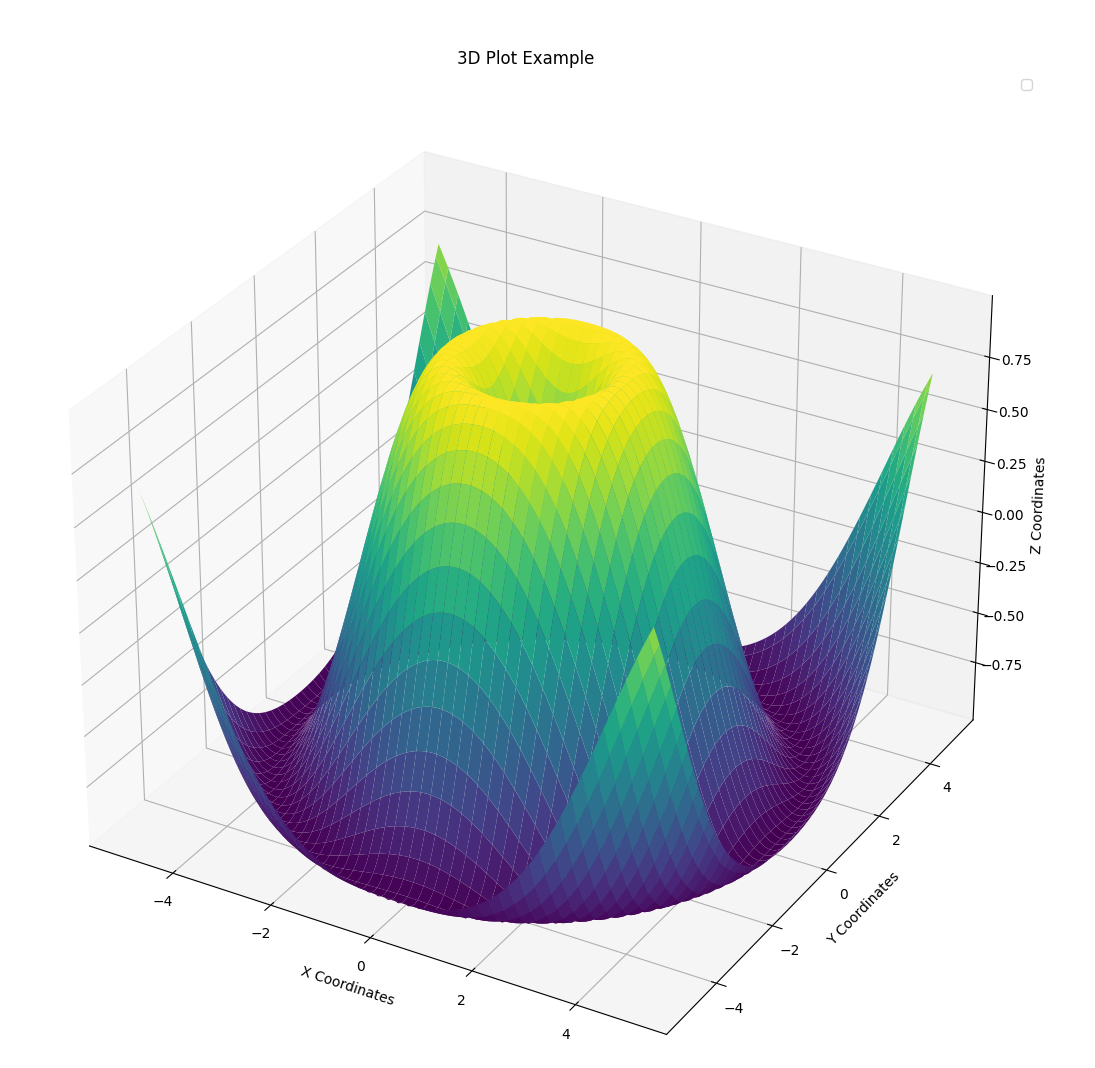
\includegraphics[width=0.65\textwidth]{fig/3dexample.png}
    \end{samepage}
\end{figure}
\end{frame}
\begin{frame}
  \frametitle{Meshgrid}
  \hrefu{https://numpy.org/doc/stable/reference/generated/numpy.meshgrid.html}{Meshgrid} is a function that returns coordinate matrices from coordinate vectors.\\
  \lstinputlisting[language=python]{examples/meshgrid.py}
\end{frame}
\begin{frame}
  \frametitle{3D - Plotting (types)}
  \begin{itemize}
    \item \texttt{projection='3d'} in \texttt{add\_subplot}
    \item \texttt{ax.view\_init(elev, azim)} to set the viewing angle
    \item \texttt{ax.plot\_surface} to plot a surface
    \item \texttt{ax.plot\_wireframe} to plot a wireframe
    \item \texttt{ax.plot\_trisurf} to plot a triangulated surface
    \item \texttt{ax.plot\_trisurf} to plot a triangulated surface
    \item \texttt{ax.contour3D} to plot contours
    \item \texttt{ax.scatter3D} to plot 3D scatter plots
    \item \texttt{ax.bar3d} to plot 3D bars
  \end{itemize}
\end{frame}

\begin{frame}
  \frametitle{Animations}
  Animations can be created using the \hrefu{https://matplotlib.org/stable/api/animation_api.html}{animation module} of matplotlib.\\
  \vspace{5mm}
  We will use the \texttt{FuncAnimation} class to create an animation of a pendulum.\\
  \vspace{5mm}
  We need parameters (time, fps), a way to calculate the position of the pendulum and a function to update the plot.\\
\end{frame}
\begin{frame}
  \frametitle{Animations}
  \lstinputlisting[language=python, lastline=11]{examples/animskeleton.py}
\end{frame}
\begin{frame}
  \frametitle{Animations (saving)}
  \lstinputlisting[language=python, firstline=12]{examples/animskeleton.py}
\end{frame}

\begin{frame}
  \frametitle{Histograms}
  Histograms can be created using the \hrefu{https://matplotlib.org/stable/api/_as_gen/matplotlib.pyplot.hist.html}{hist} function of matplotlib.\\
  \vspace{5mm}
  Often histograms are visualized with additional error bars. This can be done using the \hrefu{https://matplotlib.org/stable/api/_as_gen/matplotlib.pyplot.errorbar.html}{errorbar} function.\\
\end{frame}


%%%%%%%%%%%%%%%%%%%%%%%%%%%%%%%%%%%%%%%%%%%%%%%%%%%%%%%%%%%%%%%%%%%%%%%%%%%%

\end{document}
%%%%%%%%%%%%%%%%%%%%%%%%%%%%%%%%%%%%%%%%%%%%%%%%%%%%%%%%%%%%%%%%%%%%%%%%%%%%

%% EOF
